\chapter{Lidar data preprocessing}
\label{sect:devs02_chapter1}

\section{Dead time correction}
\label{sect::devs02_chapter1_deadtime}

\section{Trigger delay correction}
\label{sect::devs02_chapter1_triggerdelay}

\section{Background subtraction}
\label{sect::devs02_chapter1_triggerdelay}

\section{Overlap correction}
\label{sect::devs02_chapter1_overlap}

\section{Analog and photocounting signals gluing}
\label{sect::devs02_chapter1_gluing_channels}

\section{Near- and far-field signals gluing}
\label{sect::devs02_chapter1_gluing_systems}

Let's include Figure \ref{fig::figure01} as an example.

\begin{figure}[h!]
	\begin{center}
		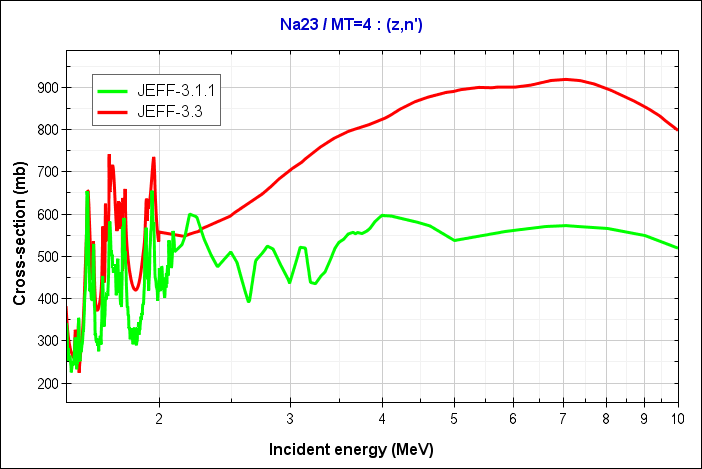
\includegraphics[width=1\textwidth]{TeX_files/Methodology/Figures/na23-mt4-XS-jeff33-jeff311.png}
		\caption{Figure caption.}
		\label{fig::figure01}
	\end{center}
\end{figure}